\section{Abelian Anyons I}

Today we discuss anyons and derive them from first principles. We focus on the 2-D case in our discussion.

\subsection{Single-particle Berry Phase}
Let $H$ be a 2-D gapped Hamiltonian with short-ranged interactions (sum of local terms). Suppose $H$ has a particle-like excitation (the rough idea is that there is a state in $\mathcal{H}$ that looks like the ground state everywhere, except for a localized region in space). In general, these excitations/particles can be in different locations in space\footnote{Physically, we could imagine these $\v{r}$ as minima of some trapping potential} $\v{r}$. For each different position, we will have a distinct many-body state, which we can label as $\ket{\v{r}}$. We can then consider the Berry phase $\theta_B(\gamma)$ associated with a closed path $\gamma$:
\begin{equation}
    \theta_B(\gamma) = \int_0^T \bra{\v{r}(t)}i\dod{}{t}\ket{\v{r}(t)}dt
\end{equation}

\begin{center}
    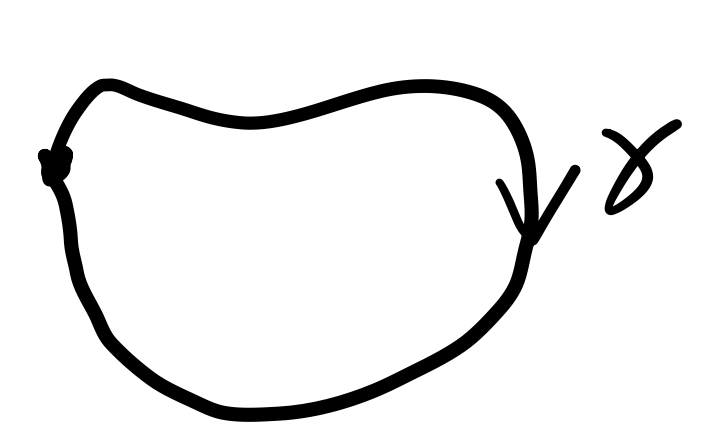
\includegraphics[scale=0.3]{Lectures/Images/lec4-path.png}
\end{center}

We can define the Berry connection, which is a vector:
\begin{equation}
    \gv{\mathcal{A}}(\v{r}) = \bra{\v{r}}i\nabla_\v{r}\ket{\v{r}} = \m{\bra{\v{r}}i\dpd{}{x}\ket{\v{r}} \\ \bra{\v{r}}i\dpd{}{y}\ket{\v{r}}}
\end{equation}
Using the chain rule, we are able to write the berry phase as an integral over the Berry connection:
\begin{equation}
    \theta_B(\gamma) = \int_\gamma\gv{\mathcal{A}}(\v{r})\cdot d\v{r}
\end{equation}
a comment; this looks a lot like a vector potential (and indeed this choice of notation is not a coincidence); the effect that $\gv{\mathcal{A}}$ has on the physics is the same as if the particle was coupled to a background vector potential/magnetic field $\v{A}$. This has very little to do with anyons - but when we go to multiple particles, we see the physics of anyons start to emerge.

\subsection{Multi-particle Berry Phase and the Locality constraint}
The extra part that appears when we look at the multi-particle Berry phase is exchange statistics (and this is how we will ``see'' anyons emerge)! Consider a state with $n$ identical excitations/particles, which we can parameterize by $\ket{\set{\v{r}_1, \ldots \v{r}_n}}$. Since the particles are identical, we need not specify the order, only the positions.

Now, let us consider the Berry phase associated with an $n$-particle closed path $\Gamma$. A picture of this path directly is a bit tricky (e.g. for 2 particles we have a 4-dimensional configuration space, which is not even Euclidean due to the lack of ordering). But we can draw it as particle worldlines through time, e.g. for four particles:

\begin{center}
    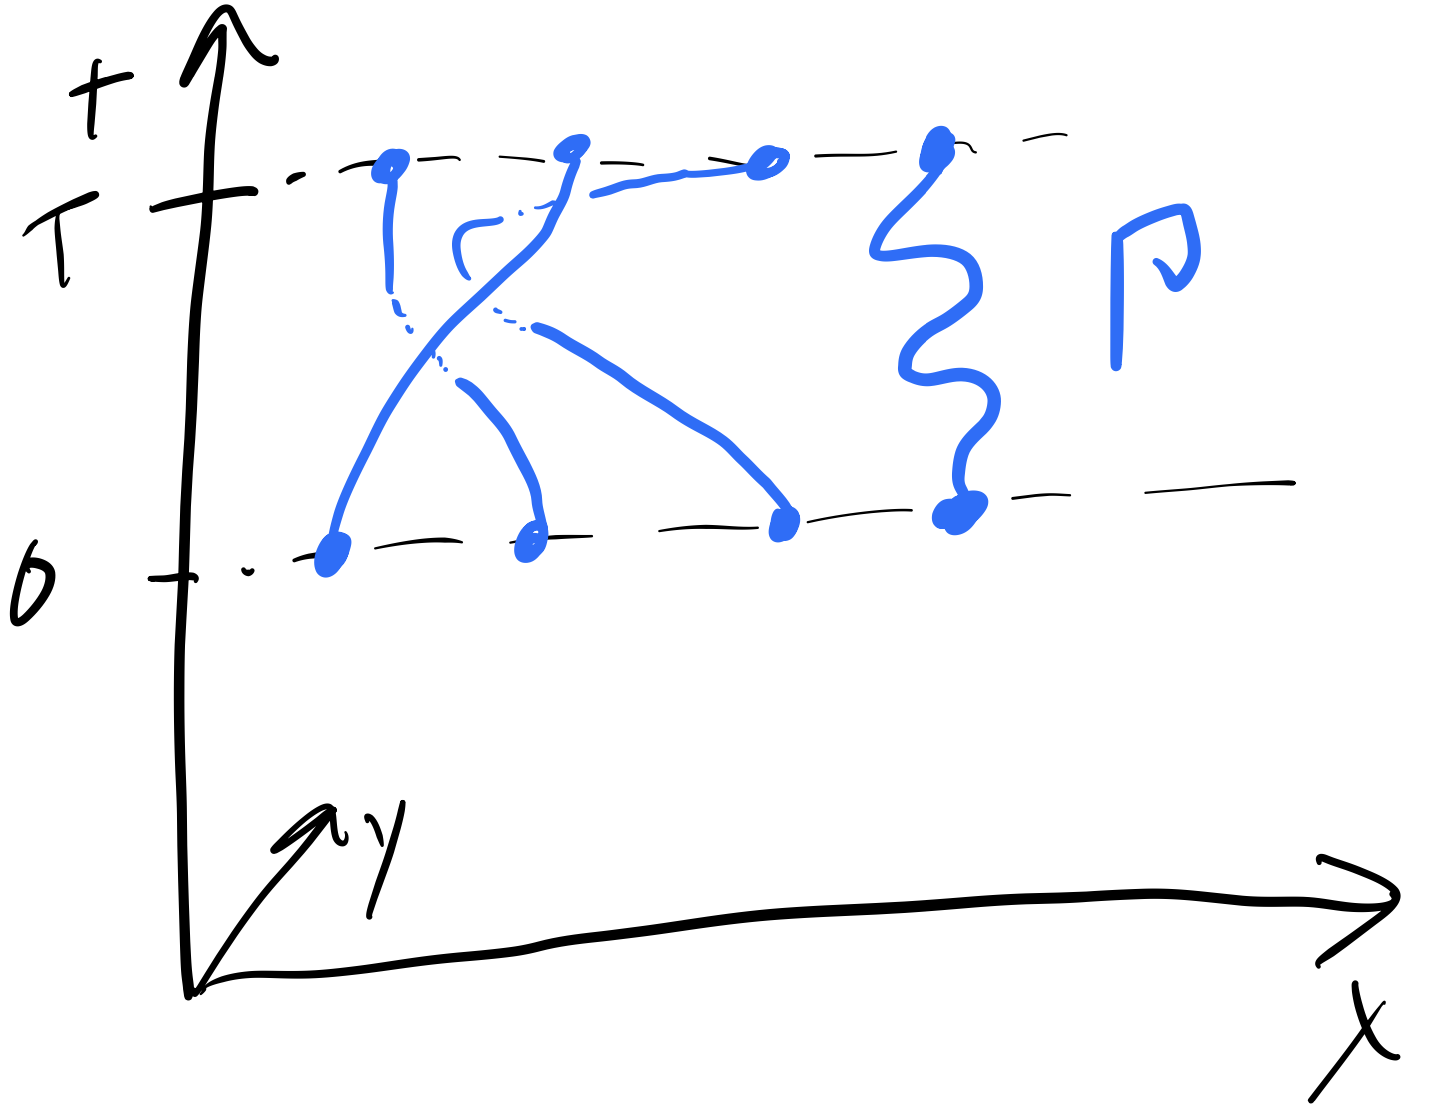
\includegraphics[scale=0.3]{Lectures/Images/lec4-worldlines.png}
\end{center}

The Berry phase is then:
\begin{equation}
    \theta_B(\Gamma) = \int_0^T \bra{\set{\v{r}_1(t), \ldots \v{r}_n(t)}}i\dod{}{t} \ket{\set{\v{r}_1(t), \ldots \v{r}_n(t)}} dt
\end{equation}
The question to understand is then; what does this look like? What are general constraints on $\theta_B$? The answer is that $\theta_B$ has to be ``local''. More precisely, imagine modifying a multi-particle path $\Gamma$ near $(\v{r}_0, t_0)$:

\begin{center}
    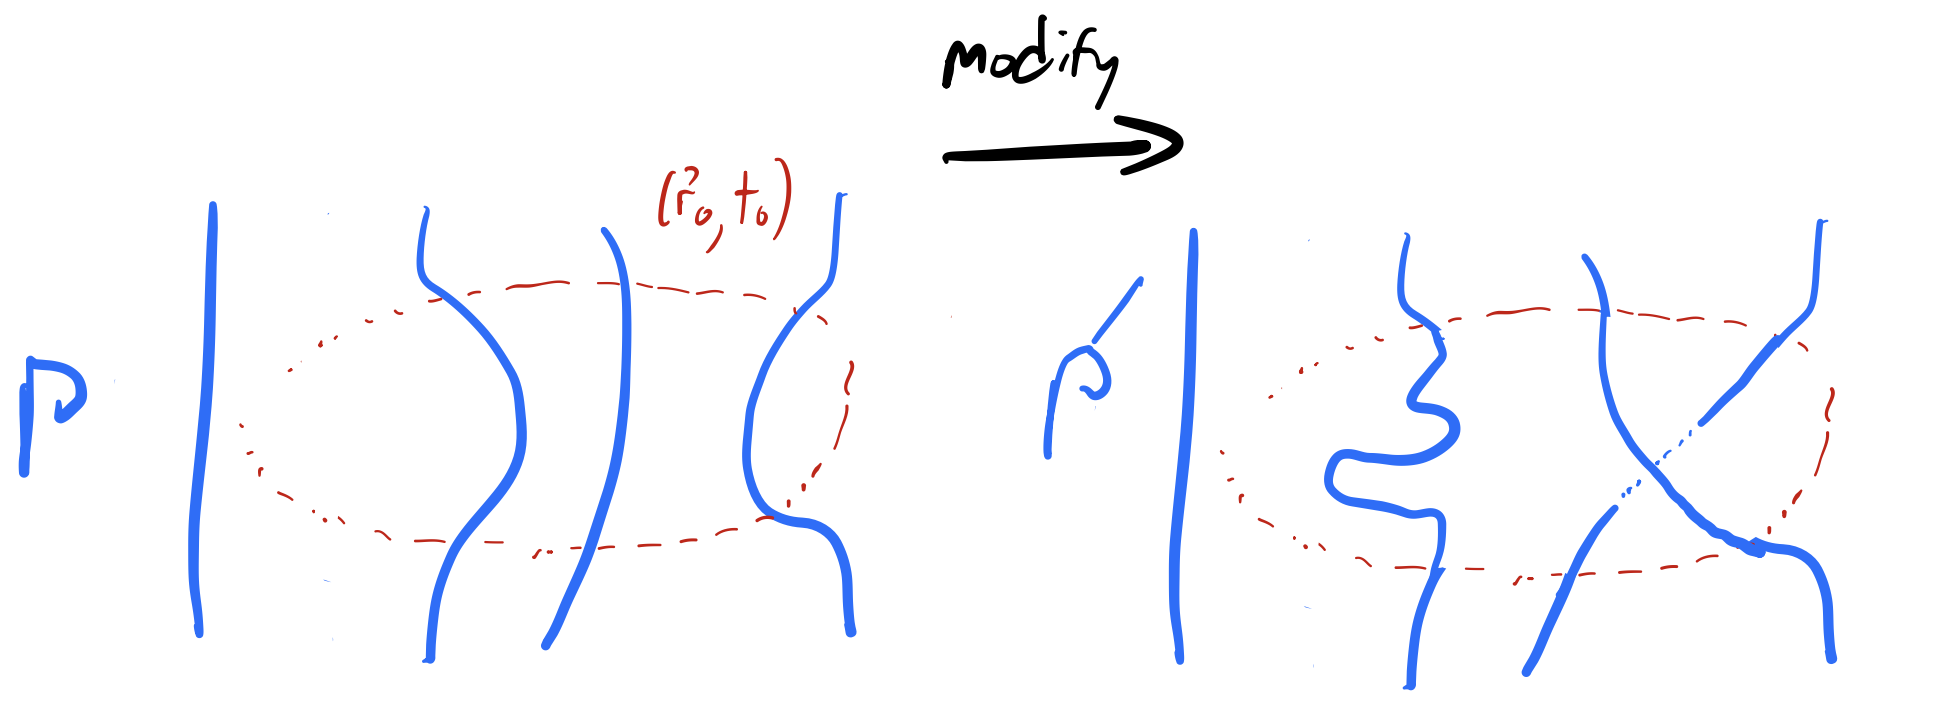
\includegraphics[scale=0.3]{Lectures/Images/lec4-localgammamod.png}
\end{center}

Then, $\theta_B(\Gamma') - \theta_B(\Gamma)$ depends only on what $\Gamma, \Gamma'$ look like near $(\v{r}_0, t_0)$. In other words:
\begin{equation}\label{eq:berryphasediff}
    \theta_B(\Gamma') - \theta_B(\Gamma) = \theta_B(\Lambda') - \theta_B(\Lambda)
\end{equation}
if $\Lambda, \Lambda'$ looks like $\Gamma, \Gamma'$ near $(\v{r}_0, t_0)$ and differ by the same local move:

\begin{center}
    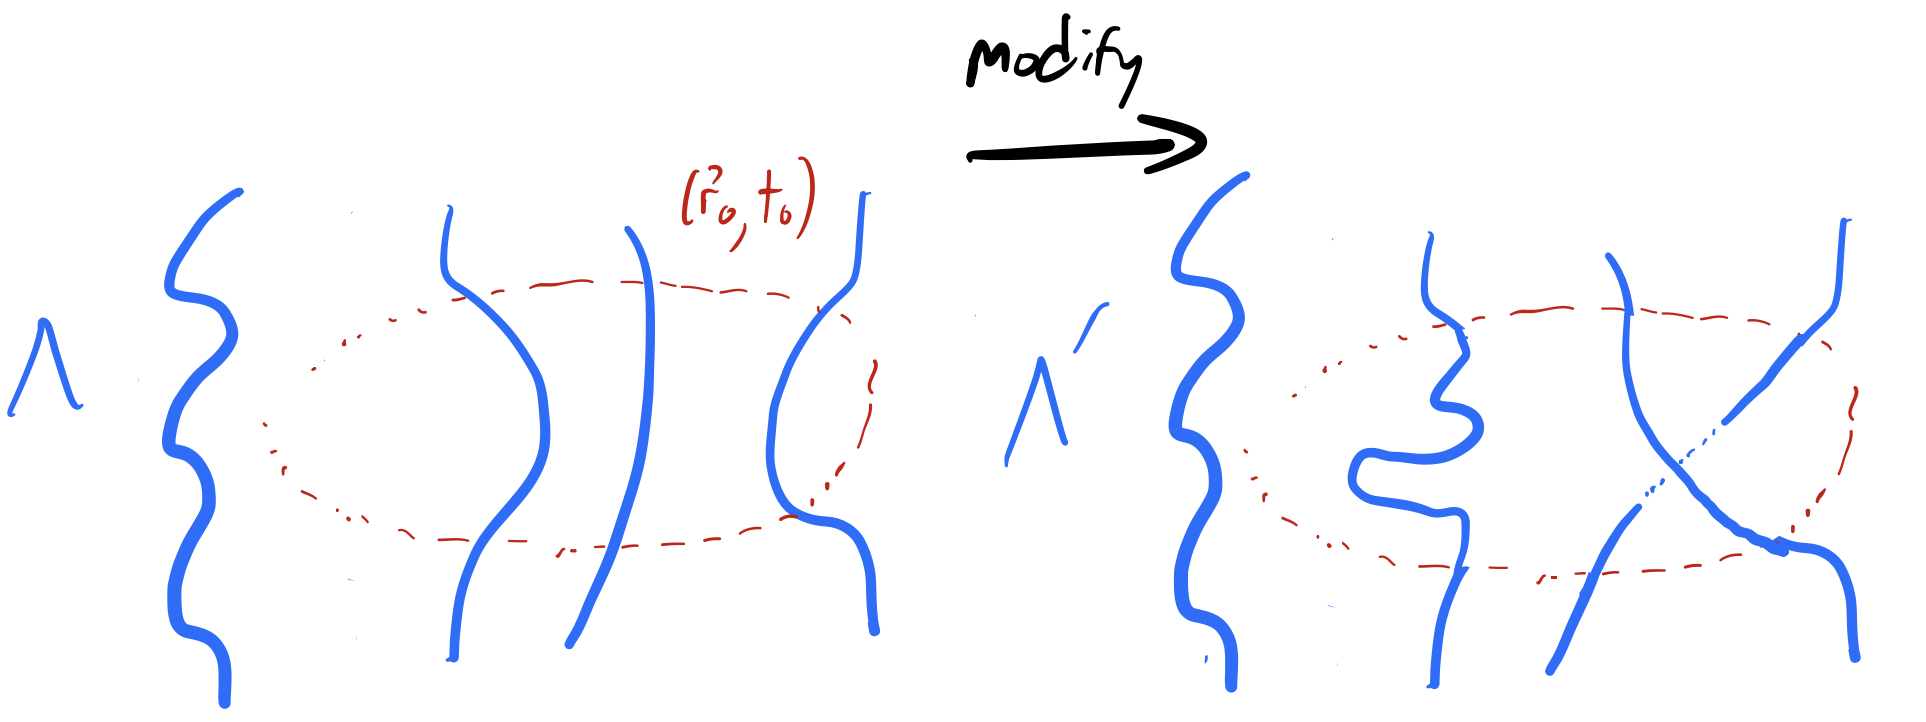
\includegraphics[scale=0.3]{Lectures/Images/lec4-localdeltamod.png}
\end{center}

The claim is local change near $(\v{r}_0, t_0)$ is insensitive to faraway modifications. Why does Eq. \eqref{eq:berryphasediff} hold? It is because the difference in Berry phase $\theta_B(\Gamma') - \theta_B(\Gamma)$ can be measured by a local operator acting near $(\v{r}_0, t_0)$ (Physically, we can imagine an interference or adiabatic experiment there). The equation then follows, assuming:
\begin{enumerate}
    \item $\ket{\Psi} = \ket{\set{\v{r}_1, \ldots \v{r}_n}}$ has short-ranged correlations, i.e.:
    \begin{equation}
        \avg{A_\v{r}A_{\v{r}'}'}_\Psi = \avg{A_\v{r}}_\Psi\avg{A_{\v{r}'};}_\Psi + \mathcal{O}(e^{-\frac{\abs{\v{r} - \v{r}'}}{\xi}})
    \end{equation}
    for $A_\v{r}, A_{\v{r}'}$ local operators supported near $\v{r}, \v{r}'$. This is where the gapped assumption comes in; the ground state of a gapped Hamiltonian has short-ranged correlations.
    \item Particles can be moved by local operators. In other words:
    \begin{equation}
        \ket{\set{\v{r}_1', \v{r}_2, \ldots, \v{r}_n}} = M\ket{\set{\v{r}_1, \ldots, \v{r}_n}}
    \end{equation}
    where $M$ is an operator supported near $\v{r}_1, \v{r}_1'$.
    \begin{center}
        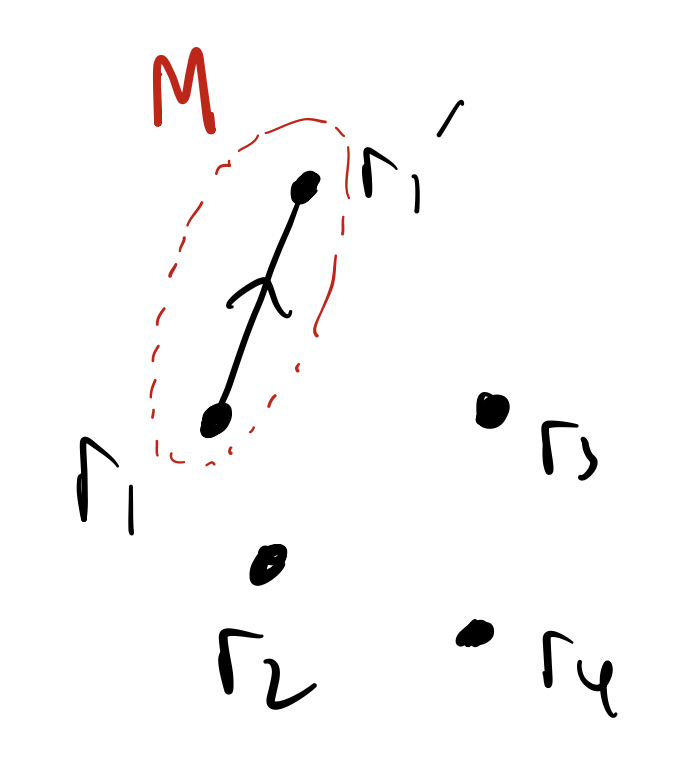
\includegraphics[scale=0.3]{Lectures/Images/lec4-Mlocal.png}
    \end{center}
\end{enumerate}
These two conditions together imply the locality constraint on the Berry phase.

\subsection{Possible Forms of the Berry Phase \& Topological Classes}
The next question is then - what is the most general Berry phase $\theta_B(\Gamma)$ that satisfies the locality constraint? One solution, and the one you probably would have guessed, is:
\begin{equation}
    \theta_B(\Gamma) = \sum_i\int_\Gamma\gv{\mathcal{A}}(\v{r}_i)\cdot d\v{r}_i.
\end{equation}
This is manifestly local. We could get a little more general:
\begin{equation}\label{eq:thetabshortrange}
    \theta_B(\Gamma) = \sum_i\int_\Gamma\left(\gv{\mathcal{A}}(\v{r}_i) + \sum_j \gv{\mathcal{B}}(\v{r}_i, \v{r}_j) + \sum_{jk}\gv{\mathcal{C}}(\v{r}_i, \v{r}_j, \v{r}_k) + \ldots\right)\cdot d\v{r}_i
\end{equation}
where $\gv{\mathcal{A}}$ is the single-particle Berry connection and $\gv{\mathcal{B}}, \gv{\mathcal{C}}$ are the two, three (and so on) particle terms so long as the multi-particle terms are short-ranged, i.e. only they are nonzero where $\v{r}_j$ is close to $\v{r}_i$ and so on. 

Is this the only possible solution consistent with Eq. \eqref{eq:berryphasediff}? No! Indeed the first proposed solution is the form of the Berry phase consistent with bosons, but there are other solutions corresponding to fermions and anyons. What does the first solution miss? Indeed it is possible to have topological terms that look highly non-local, but such that the Berry phase still has the locality constraint.

In this line, we say that two (non-intersecting) $n$-particle paths with the same endpoints are topologically equivalent if they can be continuously deformed into one another without bringing particles near each other (worldlines cannot pass through one another). For example, consider:

\begin{center}
    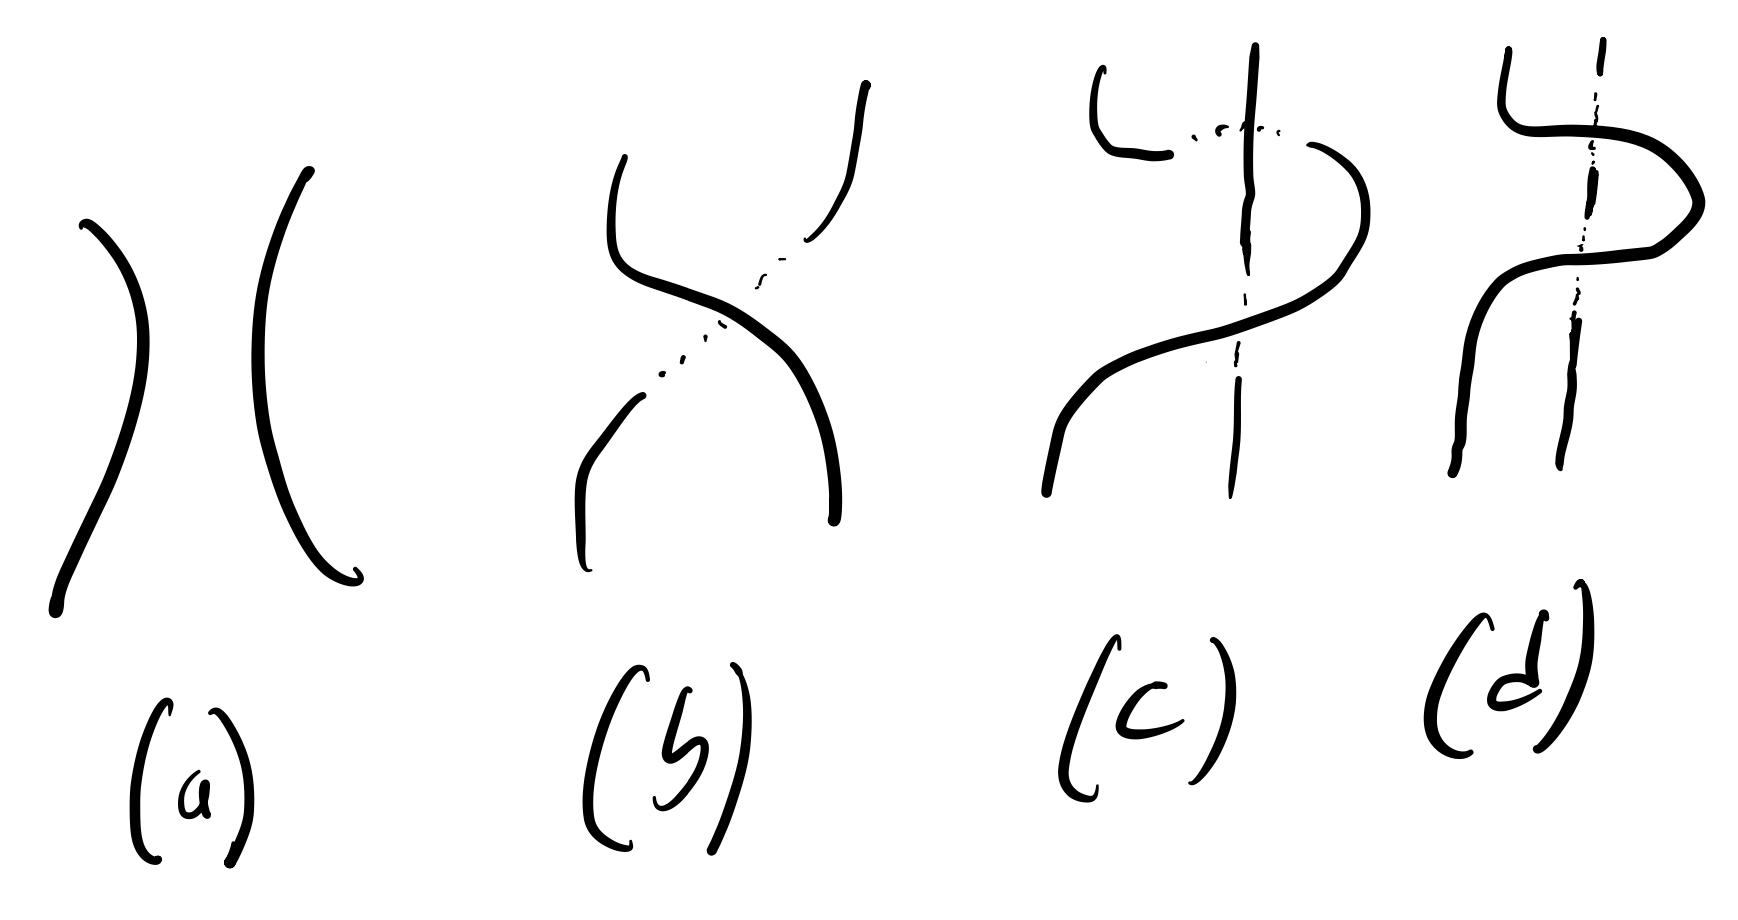
\includegraphics[scale=0.3]{Lectures/Images/lec4-topclasses.png}
\end{center}

$(a) \sim (d)$, but $(a) \not\sim (b) \not\sim (c)$. This defines an equivalence relation on (non-intersecting) $n$-particle paths, which splits the set of $n$-particle paths into equivalence (topological) classes. 

Coming back to the Berry phase, the claim is that the most general $\theta_B$ that satisfies the locality constraint Eq. \eqref{eq:berryphasediff} can be written as:
\begin{equation}\label{eq:berryphasetypes}
    \boxed{\theta_B(\Gamma) = \theta_{\text{short-range}}(\Gamma) + \theta_{\text{top}}(\Gamma)}
\end{equation}
where $\theta_{\text{top}}(\Gamma)$ only depends on the topological class of $\Gamma$ and the short-range piece is given by Eq. \eqref{eq:thetabshortrange}
\begin{equation}
    \theta_{\text{short-range}}(\Gamma) = \sum_i\int_\Gamma\left(\gv{\mathcal{A}}(\v{r}_i) + \sum_j \gv{\mathcal{B}}(\v{r}_i, \v{r}_j) + \sum_{jk}\gv{\mathcal{C}}(\v{r}_i, \v{r}_j, \v{r}_k) + \ldots\right)\cdot d\v{r}_i.
\end{equation}
Eq. \eqref{eq:berryphasetypes} is the key result. From here, we will classify the different possible topological terms we can have. We will find in 3D that we only get two possible classes and in 2D that we get many more.

Let us argue for Eq. \eqref{eq:berryphasetypes} in the special case of $\Gamma$ being a topologically trivial path, i.e. where we only have the first term. For the sake of drawing, let's look at a 2 particle path.
\begin{equation}
    \theta_B(\Gamma) = \theta_B(\gamma_1 \& \gamma_2) = ?
\end{equation}
\begin{center}
    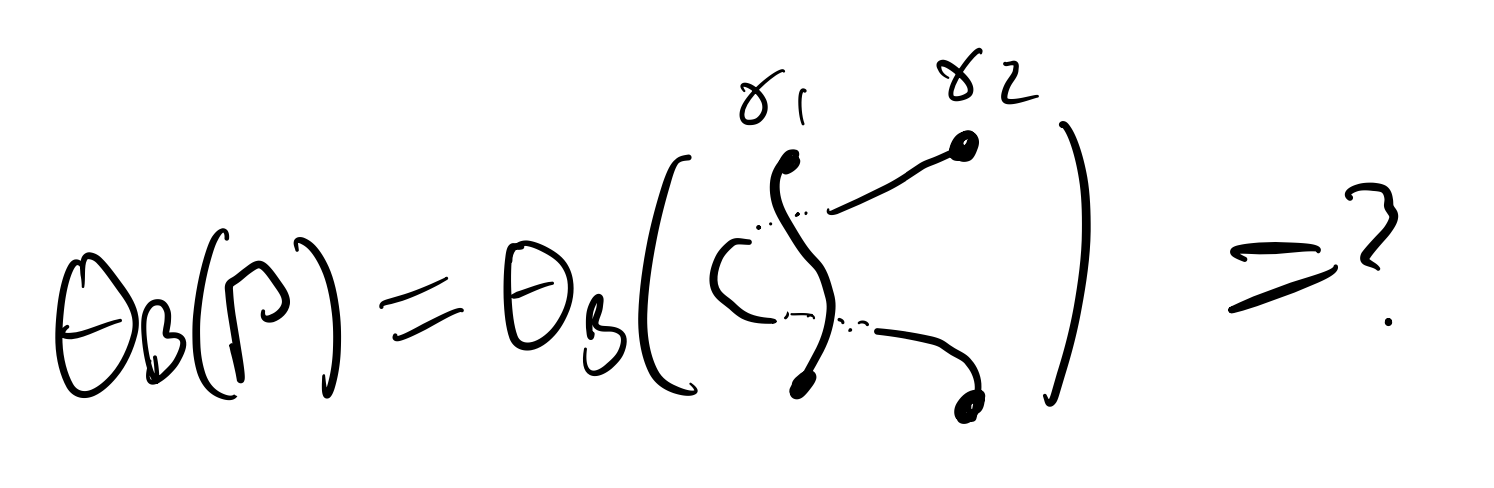
\includegraphics[scale=0.3]{Lectures/Images/lec4-thetaBtwo.png}
\end{center}
where $\gamma_1, \gamma_2$ are the single particle paths. We can then define:
\begin{equation}
    \Delta(\Gamma) = \theta_B(\gamma_1 \& \gamma_2) - \theta_B(\gamma_1) - \theta_B(\gamma_2)
\end{equation}
Now, using Eq. \eqref{eq:berryphasediff} we can use that $\Delta(\Gamma)$ is topologically invariant, i.e. it is invariant to local deformations of $\gamma_1$ far from $\gamma_2$ and vise versa. 

\begin{center}
    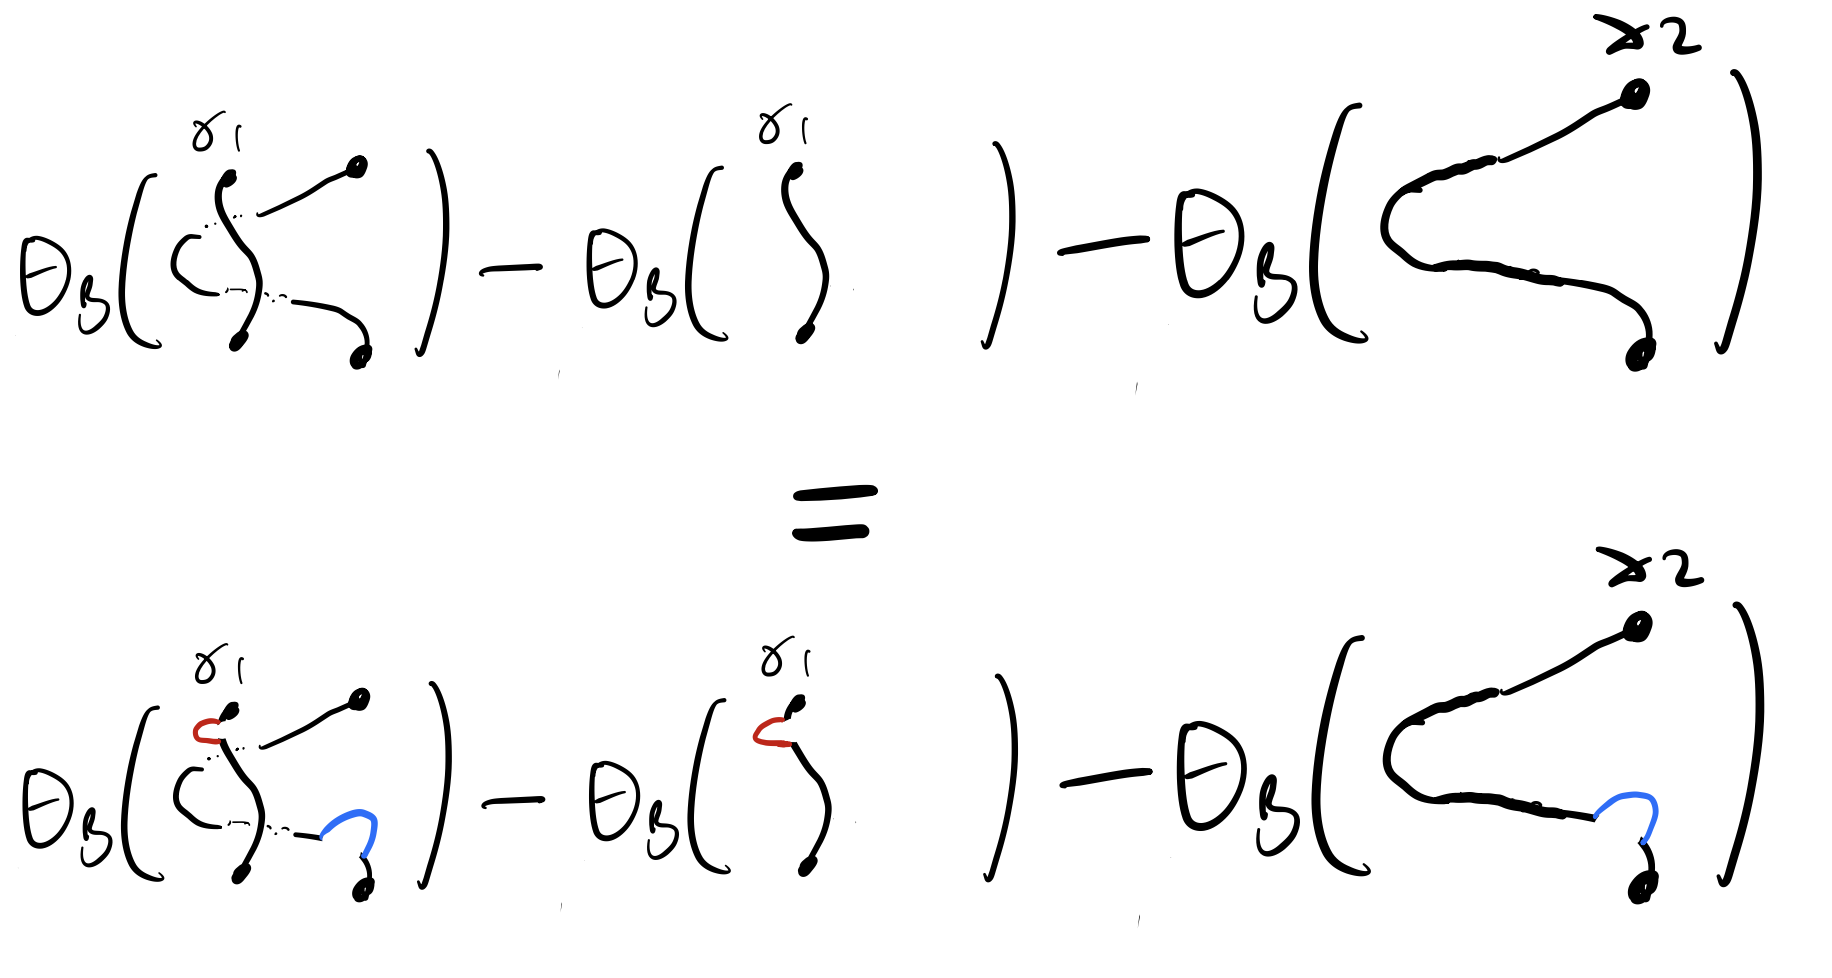
\includegraphics[scale=0.3]{Lectures/Images/lec4-thetaBequiv.png}
\end{center}

Therefore we can deform $\Gamma$ to the trivial path, for which $\Delta$ is easily seen to vanish.
\begin{equation}
    \Delta(\Gamma) = \Delta(\Gamma_{\text{trivial}}) = 0
\end{equation}

\begin{center}
    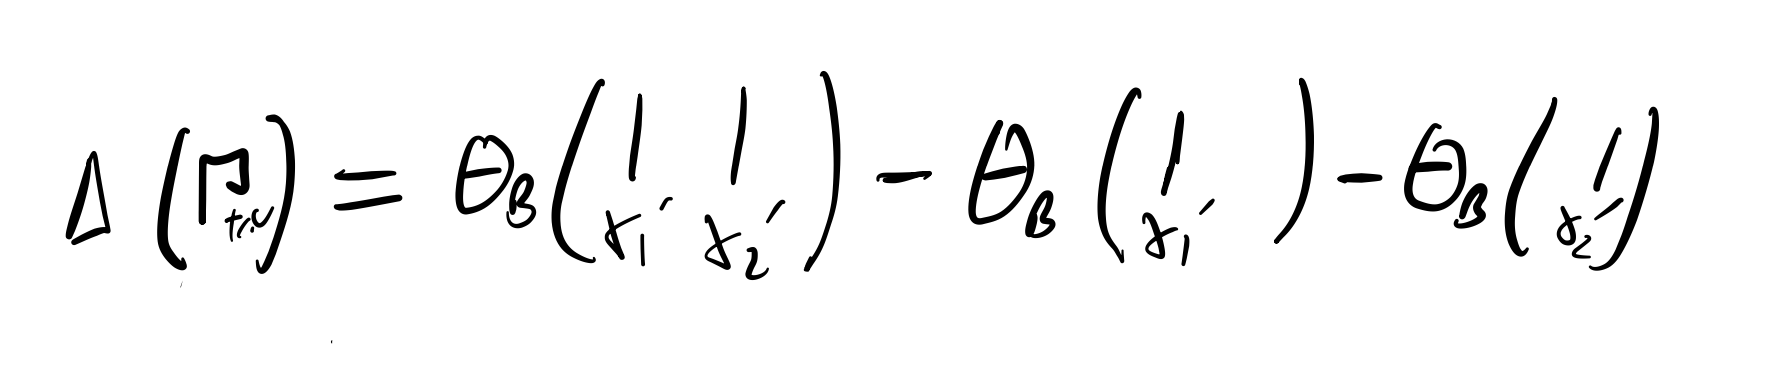
\includegraphics[scale=0.3]{Lectures/Images/lec4-thetaBtriv.png}
\end{center}

And thus since $\Delta(\Gamma) = 0$, we find:
\begin{equation}
    \theta_B(\Gamma) = \theta_B(\gamma_1) + \theta_B(\gamma_2) = \int_{\gamma_1}\v{\mathcal{A}}(\v{r}_1) \cdot d\v{r}_1 + \int_{\gamma_2}\v{\mathcal{A}}(\v{r}_2) \cdot d\v{r}_2 = \theta_{\text{short-range}}(\Gamma).
\end{equation}
